\chapter{Q-larning algoritmus}

Q-learning algoritmus je definovaný pre časovo diskrétne systémy.
Agent ktorý prechádza stavový priestor vykonaním niektorej z vopred daných
akcií získava za tieto prechody odmeny. Cieľom algoritmu je ohodnotiť všetky akcie
v jednotlivých stavoch, tak aby bol dosiahnutý ustálený stav a v každom stave
bolo možno vybrať akciu prinášajúcu najväčšiu odmenu, v globálnom zmysle.


\section{Definícia algoritmu}

Daná je množina stavov $\mathbb{S}$ a akcií $\mathbb{A}$, kde
 $\mathbb{S} \in \mathbb{R}^{n_s}$ a $\mathbb{A} \in \mathbb{R}^{n_a}$, kde
$n_s$ a  $n_a$ sú rozmery stavového vektora a vektora akcií.

Existuje prechodová funkcia
\begin{align}
        s(n+1) = \lambda(s(n), a(n))
\end{align}

zo stavu $s(n) \in \mathbb{S}$ použitím akcie $a(n) \in \mathbb{A}$, táto funkcia je ale algoritmu neznáma.

Ďalej je daná odmeňovacia funkcia $R(s(n),a(n))$, ktorá vyjadruje okamžité ohodnotenie konania
agenta v $s(n)$ a $a(n)$. V reálnych aplikáciach táto funkcia nadobúda takmer v každom
$s(n)$ a $a(n)$ hodnotu $0$. Pre správnu funkciu algoritmu, musí byť aspoň jedna hodnota
nenulová - napr. ohodnotenie dosiahnutia cieľového stavu (samotná existencia cieľového
stavu však pre algoritmus nie je potrebná).

Funkcia ohdnotení je definovaná ako

\begin{equation}
Q(s(n),a(n)) = R(s(n),a(n)) + \gamma \max_{a(n-1) \in \mathbb{A}} Q(s(n-1), a(n-1))
\label{eq:q_learning}
\end{equation}

\begin{itemize}
 \item $R(s(n),a(n))$ je odmeňovacia funkcia
 \item $Q(s(n-1),a(n-1))$ je odmeňovacia funkcia v stave $s(n-1)$ pre akciu $a(n-1)$
 \item $\gamma$ je odmeňovacia konštanta a platí $\gamma \in (0, 1)$.
\end{itemize}

Funkcia $\ref{eq:q_learning}$ definuje ohodnotenie akcií vo všetkých stavoch :
agent ktorý sa dostal do stavu $s(n)$ vykonaním akcie $a(n)$ zo stavu
$s(n-1)$ získal odmenu $R(s(n),a(n))$ a zlomok najväčšieho možného ohodnotenia ktoré
mohol získať dostaním sa do stavu $s(n-1)$, situáciu ilustruje obrázok \ref{img:q_learning}.


\begin{figure}[!htb]
\center
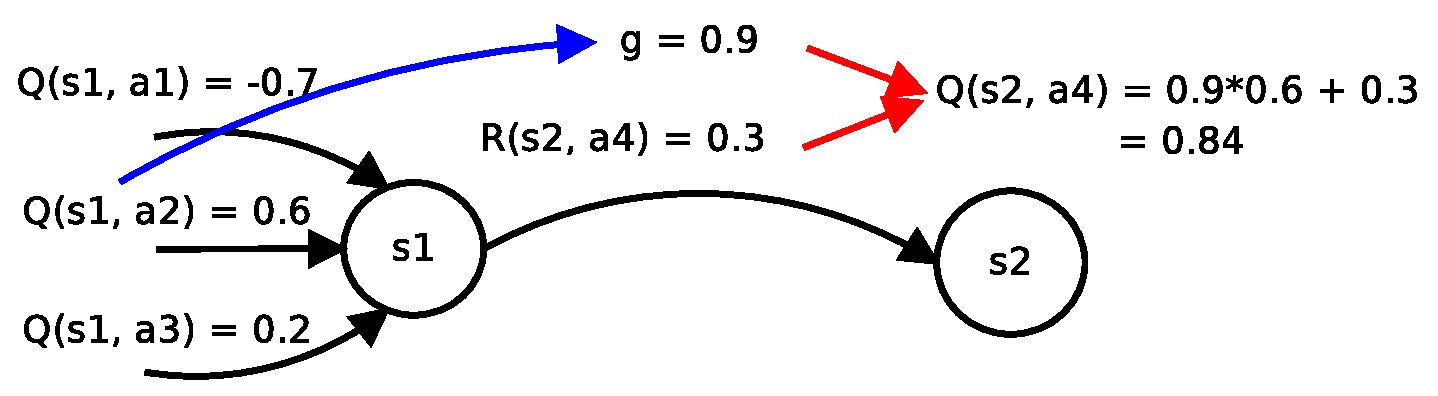
\includegraphics[scale=.6]{../diagrams/q_learning_detail.eps}
\caption{Ilustrácia funkcie ohodnotení, pre $\gamma = 0.9$}
\label{img:q_learning}
\end{figure}

Nasledujúce obrázky ilustrujú beh algoritmu pre systém so 6 stavmi.
Na začiatku nie sú známe ani samotné prechody medzi stavmi $\ref{img:q_learning_1}$, bol definovaný
1 cieľový stav $S5$, agent začína v stave $S0$ (môže však v ľubovolnom inom).
Ďalej sa pre jednoduchosť predpokladá že

\begin{equation}
R(s(n), a(a)) =
\left\{
	\begin{array}{ll}
		1  & s(n) = $S5$ \\
		0 & inak
	\end{array}
\right.
\end{equation}

t.j. odmeňovacia funkcia nadobúda hodnotu $1$ len ak sa agent dostal do stavu
$S5$.

\begin{figure}[!htb]
\center
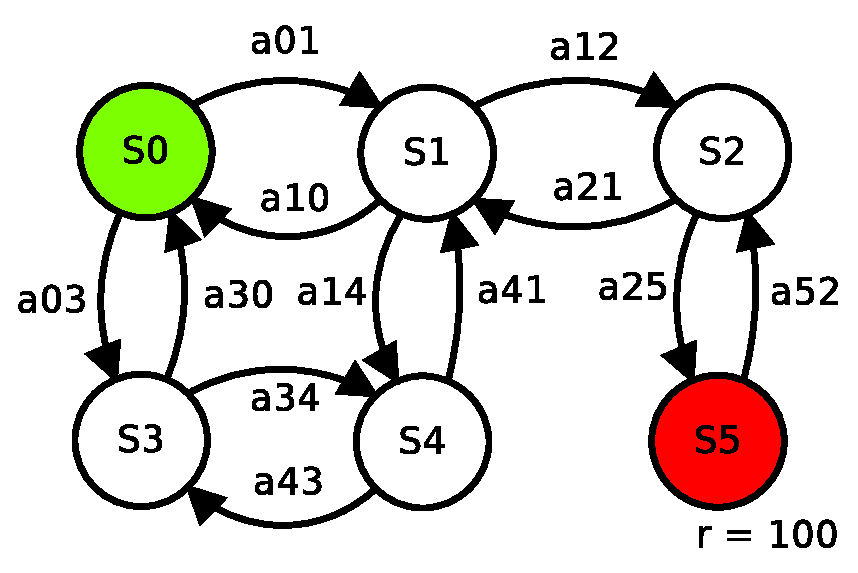
\includegraphics[scale=.6]{../diagrams/q_learning_table_01.eps}
\caption{Inicializácia}
\label{img:q_learning_1}
\end{figure}

Agent v každom stave náhodne vyberá akcie (na výbere nezáleží, dôležité je aby
každá akcia mala nenulovú pravdepodobnoť výberu, a rovnako bola nenulová
prevdepodobnosť dosiahnutia ľubovolného stavu). Obrázky \ref{img:q_learning_2}
a \ref{img:q_learning_3} ilustrujú jednu z možných ciest.


\begin{figure}[!htb]
\center
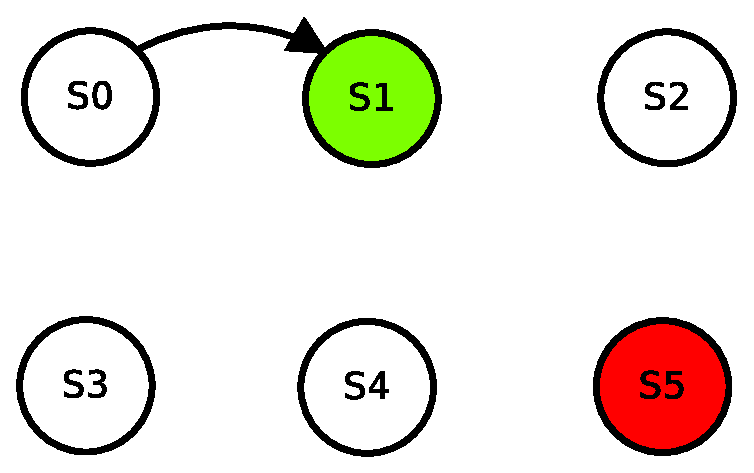
\includegraphics[scale=.6]{../diagrams/q_learning_table_02.eps}
\caption{Prechod do stavu S1}
\label{img:q_learning_2}
\end{figure}

\begin{figure}[!htb]
\center
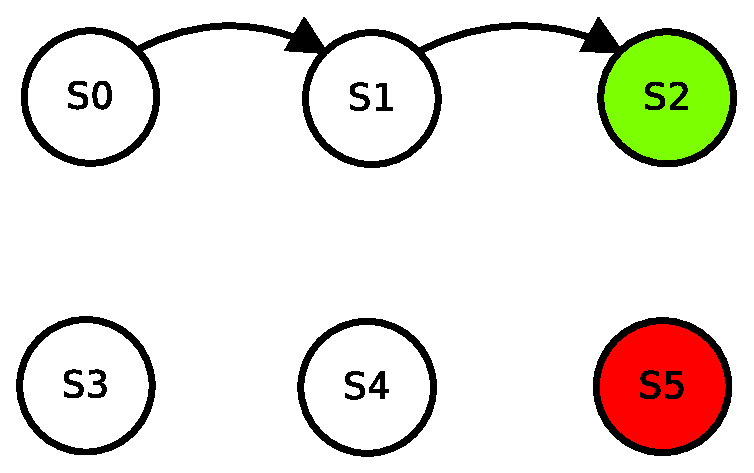
\includegraphics[scale=.6]{../diagrams/q_learning_table_03.eps}
\caption{Prechod do stavu S2}
\label{img:q_learning_3}
\end{figure}

\begin{figure}[!htb]
\center
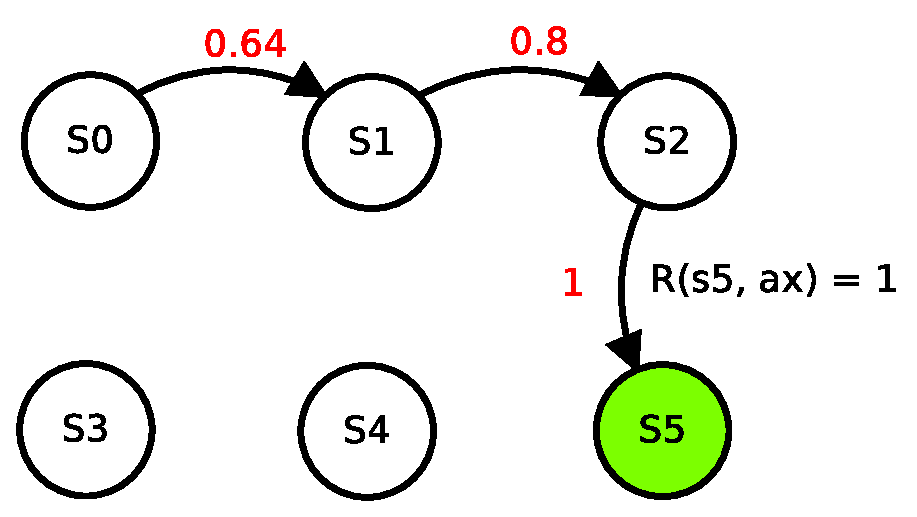
\includegraphics[scale=.6]{../diagrams/q_learning_table_04.eps}
\caption{Prechod do stavu S3}
\label{img:q_learning_4}
\end{figure}

\begin{figure}[!htb]
\center
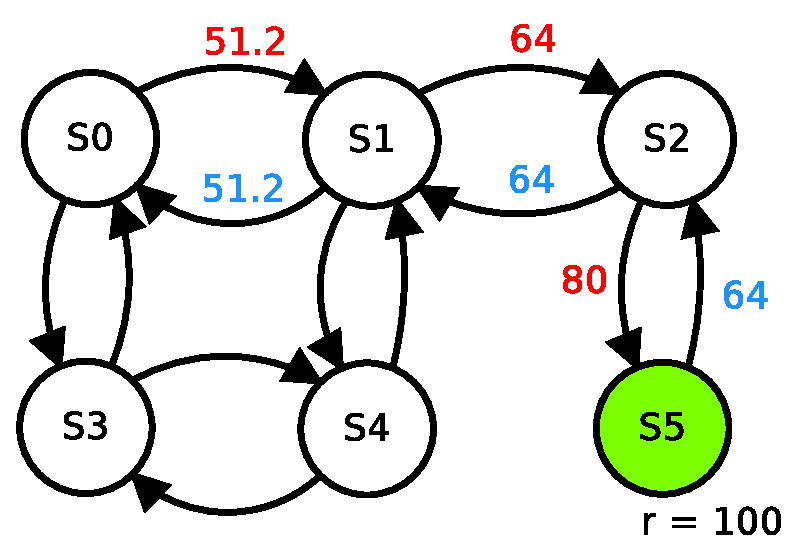
\includegraphics[scale=.6]{../diagrams/q_learning_table_05.eps}
\caption{Inicializácia}
\label{img:q_learning_5}
\end{figure}

\begin{figure}[!htb]
\center
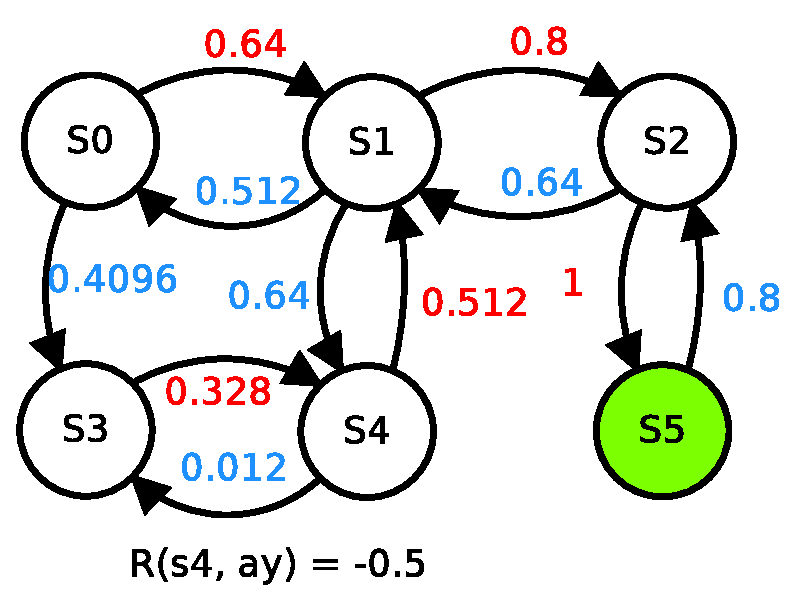
\includegraphics[scale=.6]{../diagrams/q_learning_table_06.eps}
\caption{Inicializácia}
\label{img:q_learning_6}
\end{figure}
